% Copyright (C) 2014-2017 by Thomas Auzinger <thomas@auzinger.name>

\documentclass[draft,final]{vutinfth} % Remove option 'final' to obtain debug information.

% Load packages to allow in- and output of non-ASCII characters.
\usepackage{lmodern}        % Use an extension of the original Computer Modern font to minimize the use of bitmapped letters.
\usepackage[T1]{fontenc}    % Determines font encoding of the output. Font packages have to be included before this line.
\usepackage[utf8]{inputenc} % Determines encoding of the input. All input files have to use UTF8 encoding.

% Extended LaTeX functionality is enables by including packages with \usepackage{...}.
\usepackage{amsmath}    % Extended typesetting of mathematical expression.
\usepackage{amssymb}    % Provides a multitude of mathematical symbols.
\usepackage{mathtools}  % Further extensions of mathematical typesetting.
\usepackage{microtype}  % Small-scale typographic enhancements.
\usepackage[inline]{enumitem} % User control over the layout of lists (itemize, enumerate, description).
\usepackage{multirow}   % Allows table elements to span several rows.
\usepackage{booktabs}   % Improves the typesettings of tables.
\usepackage{subcaption} % Allows the use of subfigures and enables their referencing.
\usepackage[ruled,linesnumbered,algochapter]{algorithm2e} % Enables the writing of pseudo code.
\usepackage[usenames,dvipsnames,table]{xcolor} % Allows the definition and use of colors. This package has to be included before tikz.
\usepackage{nag}       % Issues warnings when best practices in writing LaTeX documents are violated.
\usepackage{todonotes} % Provides tooltip-like todo notes.
\usepackage{hyperref}  % Enables cross linking in the electronic document version. This package has to be included second to last.
\usepackage[acronym,toc]{glossaries} % Enables the generation of glossaries and lists fo acronyms. This package has to be included last.

% Define convenience functions to use the author name and the thesis title in the PDF document properties.
\newcommand{\authorname}{Rebeka Koszticsak} % The author name without titles.
\newcommand{\thesistitle}{Enhancement of Footwear Impressions} % The title of the thesis. The English version should be used, if it exists.

% Set PDF document properties
\hypersetup{
    pdfpagelayout   = TwoPageRight,           % How the document is shown in PDF viewers (optional).
    linkbordercolor = {Melon},                % The color of the borders of boxes around crosslinks (optional).
    pdfauthor       = {\authorname},          % The author's name in the document properties (optional).
    pdftitle        = {\thesistitle},         % The document's title in the document properties (optional).
    pdfsubject      = {Subject},              % The document's subject in the document properties (optional).
    pdfkeywords     = {a, list, of, keywords} % The document's keywords in the document properties (optional).
}

\setpnumwidth{2.5em}        % Avoid overfull hboxes in the table of contents (see memoir manual).
\setsecnumdepth{subsection} % Enumerate subsections.

\nonzeroparskip             % Create space between paragraphs (optional).
\setlength{\parindent}{0pt} % Remove paragraph identation (optional).

\makeindex      % Use an optional index.
\makeglossaries % Use an optional glossary.
%\glstocfalse   % Remove the glossaries from the table of contents.

% Set persons with 4 arguments:
%  {title before name}{name}{title after name}{gender}
%  where both titles are optional (i.e. can be given as empty brackets {}).
\setauthor{}{\authorname}{Bsc}{male}
\setadvisor{Ao.Univ.Prof. Dipl.-Ing. Dr.techn.}{Robert  Sablatnig}{}{male}

% For bachelor and master theses:
\setfirstassistant{Proj.-Ass. Dipl.-Ing.}{Manuel  Keglevic}{}{male}
%\setsecondassistant{Pretitle}{Forename Surname}{Posttitle}{male}
%\setthirdassistant{Pretitle}{Forename Surname}{Posttitle}{male}

% For dissertations:
%\setfirstreviewer{Pretitle}{Forename Surname}{Posttitle}{male}
%\setsecondreviewer{Pretitle}{Forename Surname}{Posttitle}{male}

% For dissertations at the PhD School and optionally for dissertations:
%\setsecondadvisor{Pretitle}{Forename Surname}{Posttitle}{male} % Comment to remove.

% Required data.
\setaddress{Address}
\setregnumber{01325492}
\setdate{04}{01}{2020} % Set date with 3 arguments: {day}{month}{year}.
\settitle{\thesistitle}{Enhancement of Footwear Impressions} % Sets English and German version of the title (both can be English or German). If your title contains commas, enclose it with additional curvy brackets (i.e., {{your title}}) or define it as a macro as done with \thesistitle.
%\setsubtitle{Optional Subtitle of the Thesis}{Optionaler Untertitel der Arbeit} % Sets English and German version of the subtitle (both can be English or German).

% Select the thesis type: bachelor / master / doctor / phd-school.
% Bachelor:
%\setthesis{bachelor}
%
% Master:
\setthesis{master}
\setmasterdegree{dipl.} % dipl. / rer.nat. / rer.soc.oec. / master
%
% Doctor:
%\setthesis{doctor}
%\setdoctordegree{rer.soc.oec.}% rer.nat. / techn. / rer.soc.oec.
%
% Doctor at the PhD School
%\setthesis{phd-school} % Deactivate non-English title pages (see below)

% For bachelor and master:
\setcurriculum{Visual Computing}{Visual Computing} % Sets the English and German name of the curriculum.

% For dissertations at the PhD School:
%\setfirstreviewerdata{Affiliation, Country}
%\setsecondreviewerdata{Affiliation, Country}


\begin{document}

\frontmatter % Switches to roman numbering.
% The structure of the thesis has to conform to
%  http://www.informatik.tuwien.ac.at/dekanat

\addtitlepage{naustrian} % German title page (not for dissertations at the PhD School).
\addtitlepage{english} % English title page.
\addstatementpage

\begin{danksagung*}
\todo{Ihr Text hier.}
\end{danksagung*}

\begin{acknowledgements*}
\todo{Enter your text here.}
\end{acknowledgements*}

\begin{kurzfassung}
\todo{Ihr Text hier.}
\end{kurzfassung}

\begin{abstract}
\par
Shoeprint images are one of the most commonly secured evidences on crimescenes.
Even though automatic shoeprint processing is a highly researched topic, the final identifacion is usually done by human forensic experts.
The two main steps of shoeprint identification are enhancement and matching. 
\par
In this thesis the possibilities for enhancement of shoeprint samples from a real-life dataset are investigated.
The main challange of this task is to correctly filter the pattern regardless the versitile, possibly heavily structured and clutterd noise on the samples.
Two approaches are examined, pattern enhancement and noise suppression.
Among fully automated methods, a semi-automated technique is also tested, where user input is required for noise separation.
\par
The main goal of this work is to find a universal approach which is able to filter and enhance the shoeprint data even in the presence of noise and the possible low image quality.
Based on the experiences acquired while investigating the possible techniques a new noise-supression pipeline for shoeprint images is introduced.
The noisy pixels are identified based on the Fourier-Mellin features of their multi-sized neighborhood.
In the same time a model is built about the average appearance of noise, to eliminate that structure from the foreground as well.
Additionally a gradient based line detector is also applied and the edge structures of the shoeprint are clustered to distinguish between pattern and noise edges.
The experimental results show that the processed images are clearer, the pattern is sharper whereas the noise is either completely eliminated in the background or suppressed in the foreground.
Furthermore based on the results of three differenet basic image descriptor features, the enhanced shoeprints have higher matching rate to their ground-thruth samples than the original images.


\end{abstract}

% Select the language of the thesis, e.g., english or naustrian.
\selectlanguage{english}

% Add a table of contents (toc).
\tableofcontents % Starred version, i.e., \tableofcontents*, removes the self-entry.

% Switch to arabic numbering and start the enumeration of chapters in the table of content.
\mainmatter

\chapter{Introduction}

\par
Shoeprints found on crimescenes can be important hints or evidences in a criminal investigation \cite{kong2014novel}.
Event though on one thrid \cite{alexandre1996computerized} of crimescenes usable shoepatterns can be secured, there is no fully automatized algorithm available yet, which is able to identify and match those prints with the original shoe sole.
Because of that human power is needed \cite{wang2014automatic} to recognize and analyze the found patterns.
The work of forensic experts is not only time consuming and expensive, there is no guarantee about the objectivness of the final outcome\cite{gueham2008automatic}, furthermore the stages of the human matching process are unclear and not necessarily reproducible.
\par
There is an excessive amount of research already done \cite{rida2019forensic} in order to help or repleace the work of forensic experst.
There is however no algorithm published yet, which can be relaiably used in varying conditions and sample quality.
One reason for that are the already mentioned versitile conditions, the features and properties of the pattern on the shoe, like age, material, etc., the characteristics of the ground where the shoeprint is left and enviromental conditions like for example the weather highly influence the overall quality of the acquired sample.
Those high amount of factors result in changing appearance of the prints of the same shoe causing high intra class variance while clustering.
Additionally there is a lack of universal, wide ranged database \cite{rida2019forensic} which correctly depicts the common scenarios occuring on real-life crime scenes.
\par
In 2014 a new database, called FID-300 \cite{kortylewski2014unsupervised} was released which aims to solve the database problem described above.
It contains over 1000 reference shoeprint patterns acquired in a laboratory.
Moreover the database introduces 300 new shoeprint samples collected by the police providing an insight on images forensic experts are working on the daily basis.

\section{Problem Definition}
\par
There are two main stages of automatic shoeprint identification, filtering, where the shoeprint pattern is separated from background and enhanced as well, and matching where the corresponding shoe is determined.
Instead of automatizing the entire shoeprint recogition pipeline this work only focuses on the possible ways of icreasing the sample quality.
Because of the mentioned absence of general, appropiate database it is difficult to compare the already available methods.
Furthermore it is also challanging to estimate which one is applicable in a real-life scenario.
In this thesis multiple possible enhancing techniques are developed and tested in order to find a method which is able to cope with samples taken from real crime scenes.
\par
For evaluation and testing the FID-300 database is used.
The dataset contains both in a laboratory acquired as well as on a crime secured shoeprint patterns.
The goal of this work is to define an image processing pipeline which is able to correctly identify and enhance the shoepatterns and eliminate or suppress the noise on the pattern samples regardless the quality of the image.
A secondary objective is to gain an overview about the algorithms already published, and make an estimation which methods are applicable in real-life scenarios based on their performance on the FID-300 database.

\section{Challanges}
\par
There are two main obsticles in the topic of shoeprint enhancement and in automatic shoeprint matching in general, the versitile image quality and appearance and the lack of universal and wide database.
The shoeprint patterns are varying, there are approaches available which build models for given structures of the shoeprint \cite{tang2010footwear}, \cite{alizadeh2017automatic}, but no detailed, uniform representation for the entire shoeprint is possible.
Moreover there is a high inference of noise from multiple sources.
The ground where the shouprint is found is considered as noise expect in the rear case when it is left on a non changing, even surface.
The produced print of the same shoepattern varys on different type of surface.
Additionally the roughness and unevenness of a given type of surface also distorts the original pattern.
Furthermore other objects on the ground, on or behind the left shoeprint can cover or distort the original pattern, or they can prevent to leave a print on their area completely.
Besides that the pattern on the original shoe can also be distorted or modified compared to the new version.
Distortions caused by usage are valuable information about the owner, on the other hand they make it more difficult to match the pattern with their unused pairs.
Additional objects between the structures of the shoeprint also alter the original appearance.
Lastly, there are multiple shoeprint securing methods producing different results for the same print \cite{katireddy2017novel}. 
The shoeprint lifting technique used depends on the properties of the ground. 
Those two factors, the securing method and the floor, also determine if the positive or the negative, the actual pattern or the space between the shoeprint structures, image is captured.
\par
The non-existing universal database causes that two published methods are difficult to compare based on their results since they are using different testing images.
The used dataset is not necessarily published \cite{katireddy2017novel}, \cite{dardi2009texture} making it impossible to reproduce the reulst in those cases.
Additionally the handcrafted databases can be biased, and allow such restrictions and modifications which do not correlate with real-life scenarios \cite{rida2019forensic}.
The used samples are either synthetically generated and computationally distorted \cite{de2005automated}, \cite{gueham2008automatic} or exlude low quality and noisy images \cite{dardi2009texture}, \cite{tang2010footwear}.
Because of that it is difficult to compare their performance and to estimate which one of the published approaches are applicable on the FID-300 database.
Furthermore it is challanging to plan a new algorithm based on the published results because their lack of a uniform baseline.

\section{Contribution}
\par
In this thesis the possible ways of enhancing a shoeprint images are discussed.
Because of the known issues on database multiple approaches are implemented, discussed and evaluated.
The two ways to increase the quality of a given shoeprint sample is to enhance the pattern regardless of the noise and to supress or eliminate the noise without losing any of pattern information.
Along fully-automated methods semi-automated possibilities are also considered.
Three different approaches are introduced and examined for their performance on real-life image samples.
\par
Finally a new semi-autoamted framework is given which is evaluated on the FID-300 database.
In the first step user ipnut about the noise is required.
The input is separated into tiles, and the subparts are compared based on the Fourier-Mellin features to the region of the use input.
In that way the background is separated from the foreground and the average appearance of the image is calculated.
Since noise appears on the pattern as well, the distorted parts are corrected based on the calculated noise model.
After that gradient based line detection is perfromed and the results are separated into clusters where pattern and noise classes are defined and candidates of the latter are eliminated.
The final image is thresholded to create a binary image, where the shoeprint is clearly visible and recognizable whereas the clutter is supressed on the pattern and eliminated in the background of the image.
Throughout the whole processing pipeline morphological opeartions and small structure elimination is applyed multiple times.
First when a mask for background is built, and also in the end of the pipeline to eliminate small inconsistencies on the pattern.
Experimental results show, that the enhanced images are clearer, the background is successfully eliminated and the shoeprint pattern is less noisy than on the original images.
Figure \ref{fig:example} shows an example sample from the FID-300 database \ref{fig:intro:orig} and the enhanced images \ref{fig:intro:enhanced} with the proposed algorithm.
Moreover the  matching of the sample and the enhanced images with their in a laboratory lifted pair according to basic image features such as SIFT and SURF indicate that the improved images have a better matching rate than its original version.


\begin{figure}[h]
  \centering
  \begin{subfigure}[b]{0.45\columnwidth}
    \centering
    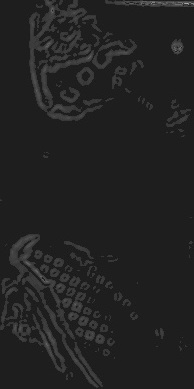
\includegraphics[width=\textwidth]{1/00182.jpg}
    \subcaption{Example image from the FID-300 database}
    \label{fig:intro:orig}
  \end{subfigure}
  \begin{subfigure}[b]{0.45\columnwidth}
    \centering
    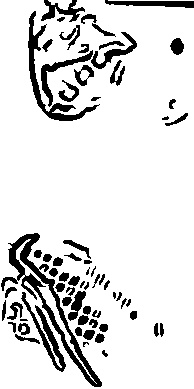
\includegraphics[width=\textwidth]{1/00182_filtered.jpg}
    \subcaption{Enhanced image}
    \label{fig:intro:enhanced}
  \end{subfigure}
  \caption{Result of the proposed algorithm}
  \label{fig:example}
\end{figure}

\section{Structure of the Work}
\par
To gain an overview about the research already done the followong section, Capter 2, gives a review about the literature. 
Along papers published in the topic of shoeprint identification, matching and enhancement, research of similar domains is presented as well.
Fields of fingerprint processing and tattoo identification is also overviewed for possibilities of using the tecniques in the given problem.
Furthermore natural image enhancement and denoising tecniques are revised as well.
\par
In Chapter 3, 4 and 5 the approaches for enhancement are given and discussed if they are applicable for real-life forensic images.
Chapter 3 presents and evaluates a possible way for pattern enhancement.
Chapter 4 and 5 describes an automated and a semi-automated noise supression pipeline respectively.
In Chapter 5 the new algorithm for enhancing real-life crimescene shoeprint impressions is proposed.
Details on implementation are revealed as well.
\par
In Chapter 6 experimental results are shown and the proposed algorithm is evaluated.
In Chapters 7 and 8 prospective future work is discussed and the final conclusion is given. 

\chapter{Related Work}
\par
In order to find and develop an effective algorithm for shoeprint enhancement an overview about relevant research has to be made first.
Along the evident litrtiture of image enhancement and noise removal a further, related topic discriminative image descriptors are also considered, to gain the best insight possible and to be able to develop an algorithm which is optimized for the rest of the shoeprint identification pipeline.
In this chapter the research on the domain of shoeprint identification is reviewed.
Other than that publications from similar domains such as fingerprint and palmprint detection as well as tattoo identification are described.
The related domains fingerprint identification and tatto recognition have been choosen for review because of their similar goal of edge structure and minimal image structure recognition.
Moreover an overview of techniques from the field of natural image enhancement and description along with general image denoising is also given.
This chapter is separated into four parts, first Image Enhancement techniques are described, after that algorithms developed for Noise Removal specifically are discussed.
In the second half of the chapter proposed methods Image Descriptors and lastly for Featuree Classifications are reviewd

\section{Image Enhancement}
\label{sec:rw:ImageENhancement}

In this section image enhancement tecniques from four specific domains are discussed, these are shoe- and fingerprint identification, tattoo recognition and natural image enhancement.

\section*{Shoeprint Enhnacement}

\par
There is an extensive research done in the field of enhancing shoeprint images.
However, it has to be noticed that the problem definition and the use-case of the different publications varys.
Becuse of the absence of standrad database, the discussed algorithms can be separated into two groups, techniques tested on synthetic samples and on real-life impressions.
Synthetic samples are images scanned in images in a laboratorial enviroment for the purpose of building a dataset for shoeprint identification.
The noise derives from scanning artifacts and computationally added distortions and modification.
Furthermore many algorithms developed for real crime-scene data make restrictions about the input image and exclude noisy and poor quality images.
Figure \ref{fig:rw:database} shows example images from a synthetic \ref{fig:rw:synthetic}, from a restricted \ref{fig:rw:restricted} and high \ref{fig:rw:highFID} and low quality samples \ref{fig:rw:lowFID} from the FID-300 dataset.
In the following discussion it is noticed repeatedly, which kind of dataset the proposed approach was tested on.

\begin{figure}[h]
  \centering
  \begin{subfigure}[b]{0.24\columnwidth}
    \centering
    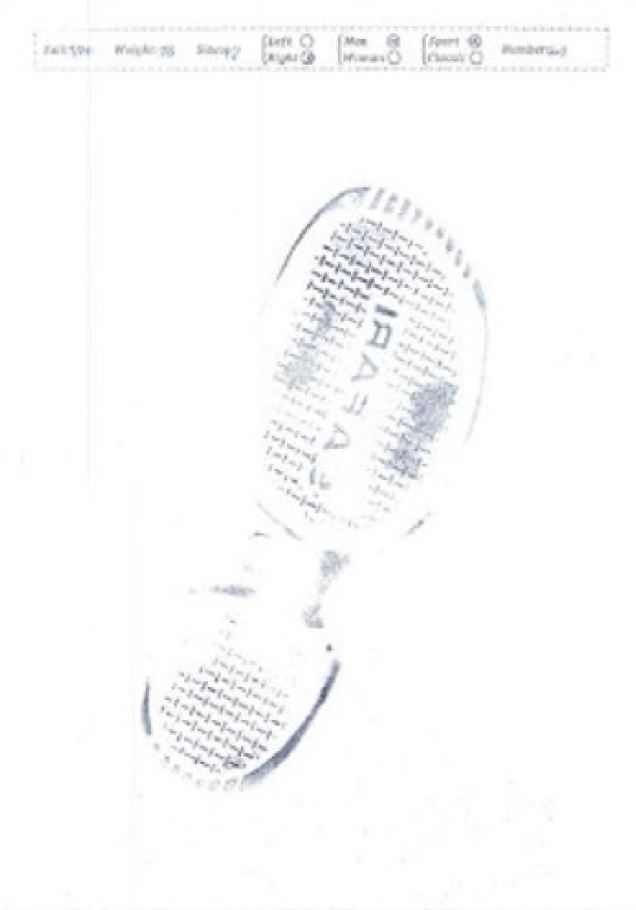
\includegraphics[width=\textwidth]{2/synthetic.jpg}
    \subcaption{Example image from a synthetic dataset}
    \label{fig:rw:synthetic}
  \end{subfigure}
  \begin{subfigure}[b]{0.24\columnwidth}
    \centering
    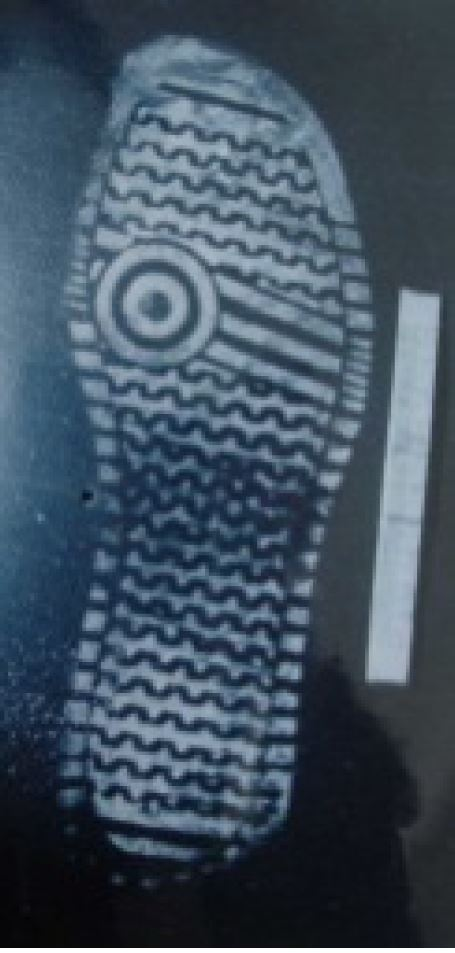
\includegraphics[width=\textwidth]{2/restricted.jpg}
    \subcaption{Example image from a real crimescene dataset exluding low quality images}
    \label{fig:rw:restricted}
  \end{subfigure}
  \begin{subfigure}[b]{0.24\columnwidth}
    \centering
    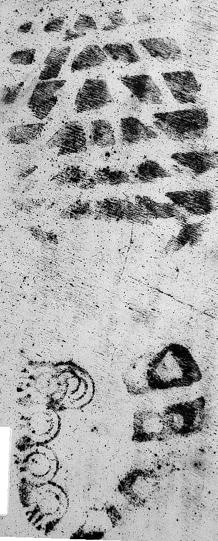
\includegraphics[width=\textwidth]{2/00025.jpg}
    \subcaption{Example high quality image from the FID-300 database}
    \label{fig:rw:highFID}
  \end{subfigure}
  \begin{subfigure}[b]{0.24\columnwidth}
    \centering
    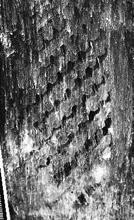
\includegraphics[width=\textwidth]{2/00174.jpg}
    \subcaption{Example low quality image from the FID-300 database}
    \label{fig:rw:lowFID}
  \end{subfigure}
  \caption{Example images of a synthetic \cite{alizadeh2017automatic}, of a restricted \cite{li2014retrieval} and of the FID-300 \cite{kortylewski2014unsupervised} dataset}
  \label{fig:rw:database}
\end{figure}

\par
Morphological Operations, Thresholding and Image Filtering are popular techniques for improve the quality of both kind, realistic and synthetic, of input data.
Morphological operations, especially Opening and Closing, is used in many cases \cite{wang2014automatic}, \cite{kong2014novel}
, \cite{li2014retrieval}, \cite{tang2010footwear}, \cite{wu2019crime}, whereas Wang et al. \cite{wang2014automatic} uses a synthetic dataset, and other than Wu et al. \cite{wu2019crime} the forensic images are restricted to high quality data.
 Wang et al. \cite{wang2014automatic}, Kong et al.  \cite{kong2014novel} and Li et al. \cite{li2014retrieval} use the Morphological Operations to correct inconsistencies after thresholding.
Similar to the previous approaches Wu et al. \cite{wu2019crime} applies the same pipeline on a real forensic dataset.
Tang et al. \cite{tang2010footwear} follow the same principle but instead of thresholding, after Canny edge detection is Opening and Closing used.
\par
To create a binary image and eliminate noise various thresholding techniques are used.
Otsu  \cite{wu2019crime}, \cite{algarni2008novel}, \cite{alizadeh2017automatic}, \cite{kong2014novel} and adaptive thresholding \cite{wang2014automatic}, \cite{li2014retrieval} are the two most popular algorithms.
Algarni et al. \cite{algarni2008novel} and Alizedah et al. \cite{alizadeh2017automatic} along with Wang et al. \cite{wang2014automatic} published their algorithms for synthetic datasets.
Kong et al. \cite{kong2014novel} and Li et al. \cite{li2014retrieval} tested on restricted, whereas Wu et al. \cite{wu2019crime} developed their approach for full real forensic database.
Wang et al. \cite{wang2014automatic} and Wu et al. \cite{wu2019crime} combine thresholding with a grid based approach to calculate exact thresholds for every subarea of the picture.
\par
An other way to eliminate noise is image filtering.
Alizadeh et al. \cite{alizadeh2017automatic} uses a simple Median filter on a synthetic dataset.
Zhang et al. \cite{zhang2005automatic} test on synthetic database as well.
They take advantage on the partial different equations approach.
In this way the edges are preserved while the background is smoothed according to a controlled curvature motion criteria. 
Katireddy et al. \cite{katireddy2017novel} uses Successive Mean Quantization Transfrom (SMQT) \cite{nilsson2013smqt} as an only step to ehnace a real-life database.
Figure \ref{fig:rw:SMQT} shows the output of the SMQT algorithm on an example image.

\begin{figure}[h]
  \centering
  \begin{subfigure}[b]{0.4\columnwidth}
    \centering
    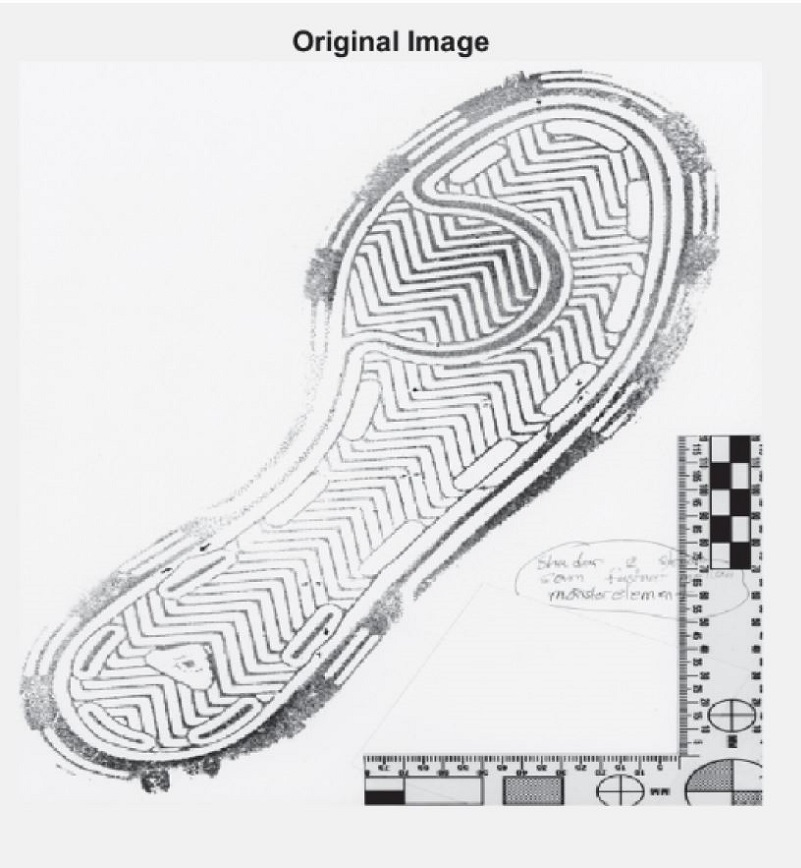
\includegraphics[width=\textwidth]{2/SMQTorig.jpg}
    \subcaption{Example shoeprint impression}
    \label{fig:rw:SMQTin}
  \end{subfigure}
  \begin{subfigure}[b]{0.4\columnwidth}
    \centering
    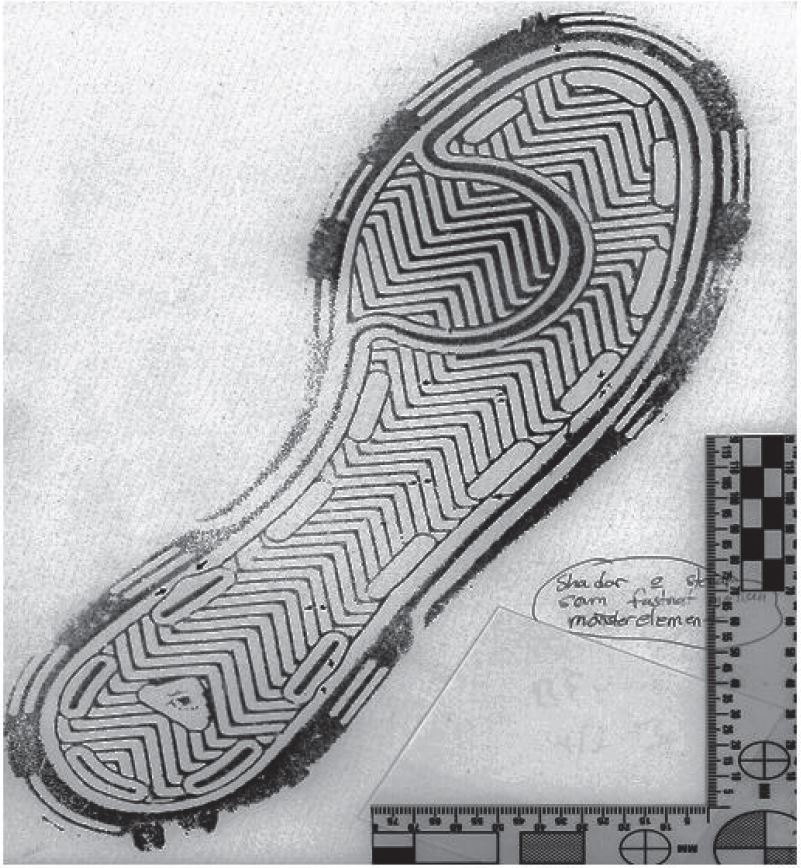
\includegraphics[width=\textwidth]{2/SMQT.jpg}
    \subcaption{Enhanced image with the SMQT algorithm}
    \label{fig:rw:SMQTout}
  \end{subfigure}
  \caption{Example image about the enhancement feature of the SMQT algorithm \cite{katireddy2017novel} }
  \label{fig:rw:SMQT} % \label has to be placed AFTER \caption (or \subcaption) to produce correct cross-references.
\end{figure}

\par
Bandpass operators are also used for noise supression.
The images are converted to the frequency domain where high and low frequencies are eliminated.
Gueham et al. \cite{gueham2007automatic} and Richetelli et al. \cite{richetelli2017classification} utilize this method on a synthetic database.
Li et al. \cite{li2014retrieval} work with a restricted real dataset, where only the lower frequencies are eliminated.
Another frequency based approach was proposed by Katireddy et al. \cite{katireddy2017novel} based on Daubechies wavelets.
After SMQT enhancement the Daubechies wavelets are used to separate the fore- and background and to remove the noise in the latter.

\section*{Fingerprint Enhnacement}

Bandpass and general image filtering is popular in the field of fingerprint enhancement as well.
Zhou et al. \cite{zhou2011adaptive} uses a low- and a highpass filter to eliminate striking frequencies. 
Baig et al. \cite{baig2015enhancement} apply Directional Hilbert transform of a Butterworth andpass to collect the different phase shifts and eliminate the artifacts created by previous thresholding of the input.
Wang et al. \cite{wang2014enhanced} decompose the image into four subbands and process them separately, calculating the noise for every subband respectively.
Li et al. \cite{li2012texture} use Fourier transformation combined with Scale Invariant Feature Transform (SIFT) to enhance the fingerrint images. \todo{reference}
With SIFT the intresting points in the Fourier domain are found and secured, while the image is filtered to suppress noise and other inconsistencies.
Jahan et al. \cite{jahan2017robust} apply Fuzzy filtering followed by thinning.
Fuzzy filter is a local method to preserve the edge information and fine lines structures and supress the noisy background of the input.

\section*{Tattoo Enhnacement}

For tattoo enhancement an algorithm from Han et al. \cite{han2013tattoo} was proposed which combines Gaussian filtering with Hysteresis thresholding. \todo{reference}
Hysteresis thresholding is a neighborhood-aware approach where a pixel is labelled when it is above a given low threshold and simultaneously connected to other pixels meeting a higher thresholding criteria. \todo{reference}
Acton et al. \cite{acton2008matching} propose to use an Active Contour Model to find the boundaries of tattoo images and apply Opening and Closing as well to get rid of small inconsistencies.

\section*{Natural Image Enhnacement}
\par
Along Signal, especially Bandpass, general Image Filtering and Thresholding Histogram and Color Operations are also common for natural image enhancement.
Maini et al. \cite{maini2010comprehensive} published a review about natural image enhancing algorithms and defined two main groups of algorithms, Frequency and Spatial Domain Methods.
First publications utilizing techniques from the first group are discussed, after that the usage of Spatial Domain Methods is reviewed.
\par
Xu et al. \cite{xu2016image} combines Bandpass filtering with adaptive thresholding.
Similar to Wang et al. \cite{wang2014enhanced} the image is separated into four subbands, and the threshold is calculated for every image separately.
Sugamya et al. \cite{sugamya2016image} applies Subband Decomposition with two staged Histogram Equalization.
The histogram of the input is equalized gloablly first, after that it is decomposed into subbands to Equalize the values locally for every four generated subimage.
\par
Median Fiters are used for noise suppression no only in the domain of shoeprint enhancement \cite{alizadeh2017automatic} but also for natural image processing.
Apart from Median Filter Li et al. \cite{li2014rapid} utilize Average and Wiener Filter as well to suppress the occuring noise and to prepare the input for neighborhood based feature extraction.
Feng et al. \cite{feng2011bag} proposed a Bag-of-Words algorithm based on the Gabor wavelets of the input. 
For preprocessing the Watershed Transform is used.
\par
Histogram Operations can be combined with not only Bandpass filtering as Sugamya et al. \cite{sugamya2016image} do but also with Thresholding as proposed by Yao et al. \cite{yao2016image}.
Their aprroach separates the histogram of the input into two parts according to Otsu\'s method.
After that the histogram is equalized of the generated subimages.
Figure \ref{fig:rw:BHNMT} shows the results of algorithm on an example image.

\begin{figure}[h]
  \centering
  \begin{subfigure}[b]{0.4\columnwidth}
    \centering
    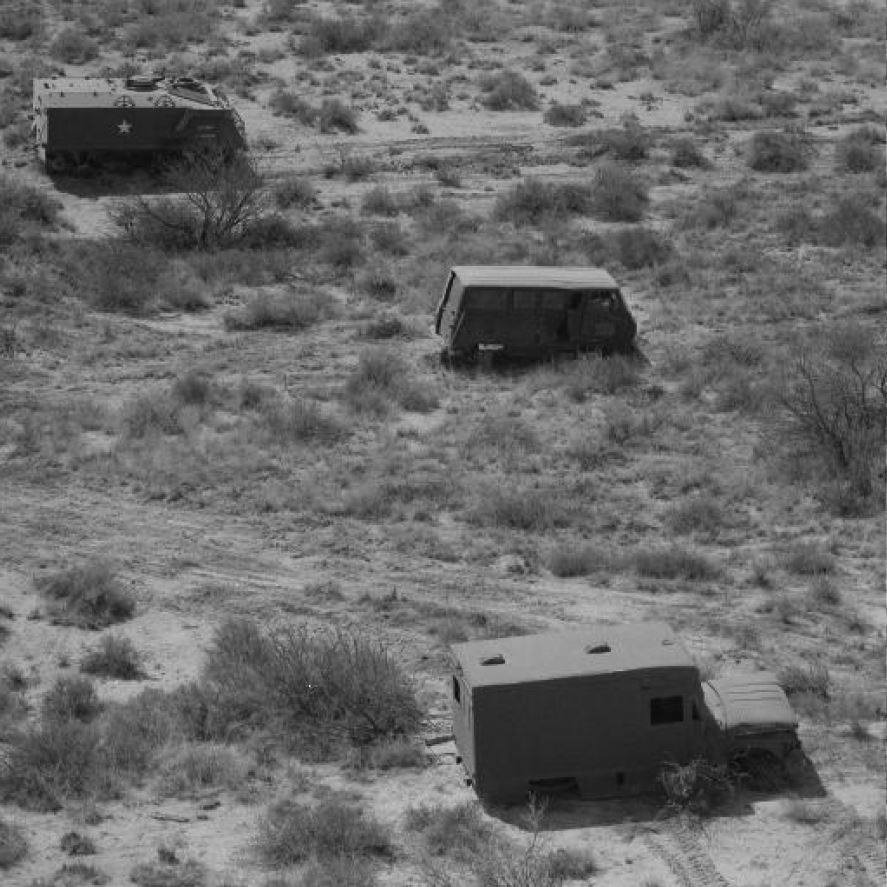
\includegraphics[width=\textwidth]{2/BHNMTorig.jpg}
    \subcaption{Example low-contrast image}
    \label{fig:rw:BHNMTin}
  \end{subfigure}
  \begin{subfigure}[b]{0.4\columnwidth}
    \centering
    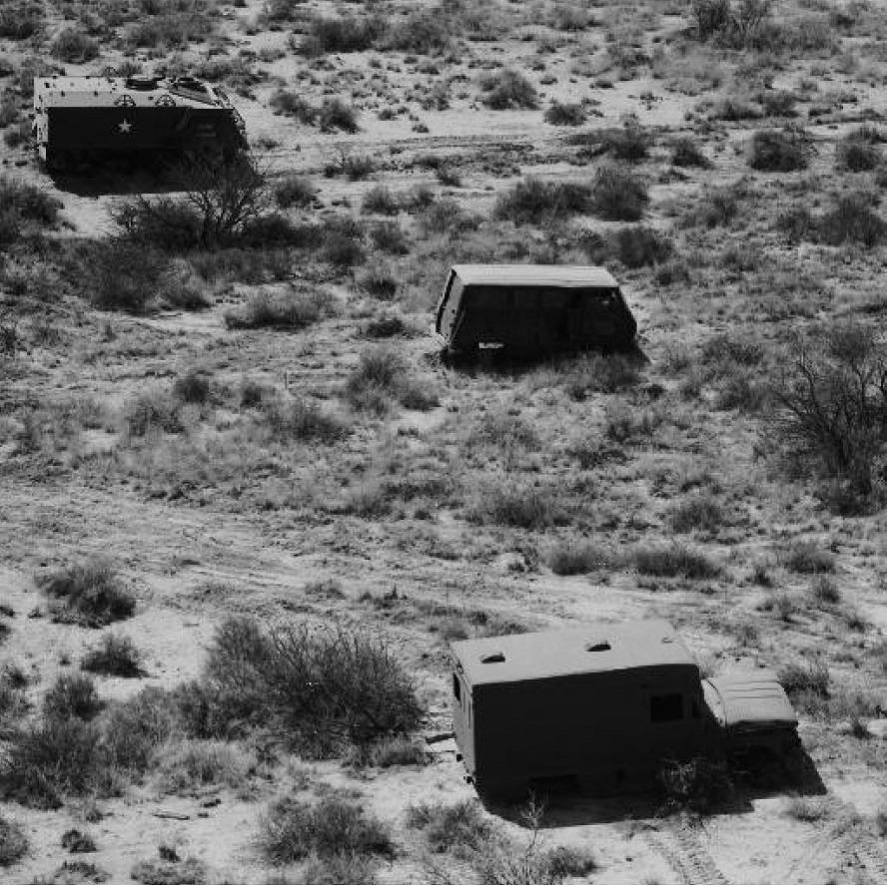
\includegraphics[width=\textwidth]{2/BHNMT.jpg}
    \subcaption{Enhanced image with the histogram thresholding algorithm}
    \label{fig:rw:BHNMTout}
  \end{subfigure}
  \caption{Example image  \cite{yao2016image} about the enhancement feature of the algorithm proposed by Yao et al. \cite{yao2016image} }
  \label{fig:rw:BHNMT} % \label has to be placed AFTER \caption (or \subcaption) to produce correct cross-references.
\end{figure}

\par
Color processing techniques are widespresd in he topic of natural image enhancement.
It can be used for image dehazing, so for low contrast images, \cite{singh2018dehazing} and also for classical noise removal \cite{ren2018joint}, \cite{zhang2016simultaneous}. 
Bhairannawar et al. \cite{bhairannawar2017color} switch from RGB to HSV and use Laplace filter to detect regions with intensity changes. 
During processing the H chanel is not modified to prevent color distortion artifacts.
Althoug color processing is a well researched field with many promissing solutions, no wider overview is given in this thesis.
There are shoeprint impression datasets with colored samples, FID-300 provides grayscale images thus no color processing approach can be used in this specific case. 

\section{Noise Removal}

Noise Removal methods are based on estimating the original image, and based on that eliminating the deviating features of the data.
One way is denoising through gradient histogram preservation \cite{zuo2013texture}.
The distribution of gradients is estimated on the original image, and the noisy image is adjusted to the calculated values.
An alternative way is to decompose a single image and based on the clear parts the noisy regions are approximated.
Huang et al. \cite{huang2013self} propose a self-learning algorithm, which only consideres the high frequency parts of the decomposed image.
There were several approaches published, where the images is separated is separated spatially instead of in the frequncy domain.
\cite{xu2015patch}, \cite{talebi2013global}, \cite{chatterjee2011patch} and \cite{guo2015efficient} are tecniques based on the idea of non-local means, where the image is subsampled into tiles and the pixels are set to the mean of regions belongng to the same cluster.
The main difference between the previous algorithms is how they classify the image subregions into different classes.
Taleby et al. \cite{talebi2013global} uses an iterative shrinkage strategy. 
Chatterjee et al.  \cite{chatterjee2011patch} groups the geometrically similar regions and estimate the noise for every class separately with a Wiener Filter.
Whereas Guo et al. \cite{guo2015efficient} utilize Block Matching to determine the cluster memberships. 
Additionally the spatial location is also considered while calculating the mean value in a given class.
The members are weighted according to the distance to the current region.

\section{Image Description}

Similar to the previous Image Enhancement section \ref{sec:rw:ImageENhancement} this part is also subdivided into four domains offering solutions for the same problem in different domains.
In this section the published image features are described which are proposed to be the most discriminative for their field.
Similar topics are reviewd to gain insight about the most powerful descriptors and consider to port them into the domain of this thesis.
Shoeprint descriptors are described first, after that fingerprint features are discussed.
Following that an overview about tattoo and natural texture descriptors is given at the end.

\section*{Shoeprint Descriptors}
\par
In the research of Shoeprint Identification and more exactly Shoeprint Description the varying difficulty and quality of the different datasets is a continuous issue, therofore the properties of the database the given approach was tested on is noted repeatedly.
Signal or frequency domain based image features are popular in both groups of algorithms using synthetic or real samples for testing.
Gabor Transform is used in several applications tested on synthetic \cite{patil2009rotation}, on restricted \cite{kong2014novel}, \cite{li2014retrieval} and on real forensic data \cite{wu2019crime} as well.
Patil et al. \cite{patil2009rotation} propose to use the Radon transfrom to determine the dominant direction of structures on the print and process the aligned image with the Gabor Transform.
Kong et al.  \cite{kong2014novel} combined the Gabor Feature of the sample with Zernike Features to describe the shapes in the pattern.
Li et al. \cite{li2014retrieval} suggest to use the histogram extracted in the Gabor Transform domain as descriptors.
In the approach published by Wu et al.  \cite{wu2019crime} Gabor Filters are combined with Haar Wavelets and Fourier-Mellin Transform to get an integratet, multi-level descriptor. 
There are other publications along with  Wu et al.  \cite{wu2019crime} where Fourier-Mellin Transfrom is proposed for feature description.
Gueham et al. \cite{gueham2008automatic} use the classical Fourier-Mellin pipeline to compare samples from a synthetic dataset.
As Wang et al. \cite{wang2014automatic} state, Fourier-Mellin transform allow multi resolution matching, so they apply it successfully on synthetic data.
Richetelli et al. \cite{richetelli2017classification} classify synthetic shoeprint impressions by applying Fourier-Mellin transform following the calculation of Phase Only Correlation (POC) to determine the translative difference between two images in the frequency domain.
Gueham et al. \cite{gueham2007automatic} in an other paper suggest to use the basic Fourier transfrom before calculating the POC.
Unlike the approach of Gueham et al. \cite{gueham2007automatic}, which were only tested on synthetic images, Kortylewsky et al. \cite{kortylewski2014unsupervised} propose a Fourier Transformation based method for real forensic images.
It is an unsupervised learning approach, where the periodic structuren on a shoeprint are compared in the Fourier domain.
Richetelli et al. \cite{richetelli2017quantitative} compares Randomly Acquired Characteristics of shoeprints, e.g. small demages, modifications and stuck objects on or in the shoesole pattern, examining their Fourier descriptor.
Othet than Fourierlike tarnsformations the use of Power Spectral Density was also proposed for a restricted dataset \cite{dardi2009texture}.
It is a descriptor for random, broadbrand signals based on the frequency and power.
\par
In high quality datasets shape descriptors are a popular choice for feature extraction.
Algarni et al. \cite{algarni2008novel} suggest to use Hu moments because of its robustness against noise, rotation and resolution.
For restricted databases it is proposed to combine the feature descriptors, Kong et al. \cite{kong2014novel} incorporate Zernike and Gabor features whereas Tang et al. \cite{tang2010footwear} define their own fundamental shapes based on common basic structures on a shoesole through Hough Line Transfrom.
The extracted features are then stored in an Attributed Relational Graph to represent the entire shoeprint image.
\par
SIFT and Harris Detector are the two most popular point descriptors for matching shoeprint images.
Nibouce et al. \cite{nibouche2009rotation} propose to use a four-level Harris and combine with SIFT on a synthetic database.
Almaadeed et al. \cite{almaadeed2015partial} use the same combination and the Hessian Detector additionally for the same purpose on a restricted real-life dataset.
Another publication \cite{richetelli2017classification} extract the SIFT features from the frequency domain after applying Fourier-Mellin Transformation and POC on the input image.
\par
Kong et al. \cite{kong2017cross}, \cite{kong2019cross} define a new descriptor for real database extracting the mid-level features from a Convolutional Neural Network.
Wu et al .\cite{wu2019losgsr} also use machine learning to calculate opinion scores for given matching pairs from real forensic data.
In the learning process manifold ranking is used where he opinions of humanexperts as well as feature similarities are both incorporated.
Kortylewsky et al. \cite{kortylewski2016probabilistic} developed hieararchical composition for Active Basis Models for the same real database, FID-300, as used in this thesis, and also extended for natural image enviroments \cite{kortylewski2019greedy}.
Sparse representation was also proposed \cite{alizadeh2017automatic} this method however was only tested on synthetic data and not on real forensic dataset.

\section*{Fingerprint Descriptors}
\par
Signal domain representations, because of their robustness against rotation, are attractive not only for shoeprint but also for fingerprint description.
Multi-resolution representation through Gabor expansion was proposed by Bolle et al. \cite{bolle2012fingerprint} to get a localized texture descriptor.
Van et al. \cite{van2016fingerprint} use Adaptively Adjusted Modified Finite Radon Transform after Gabor filtering to connect edges and eliminate inconsistencies.
Rida et al. \cite{rida2018palmprint} propose an ensambe descriptor consisting of Gabor filter, Local Binary Pattern, Histogram of Orinted Gradient (HOG) and Line detector to represent a palmprint impression.
Other than that Li et al. \cite{li2012texture} suggest to use Directional Filter Banks along, where the image is separated into eight directions and every subimage is decomposed into two frequencies vie wavelet transform.
\par
Unlike in the domain of shoeprint image representation, in case of fingerprint images several point feature descriptors were proposed.
In \cite{zhou2011adaptive} SIFT features were fused with Hough Transform and Minutiae Information of the fingerprint.
Chen et al. \cite{chen2013hierarchical} also use the Hough Transform and extends with hierarchical voting score to get better matchin information.
Along  \cite{rida2018palmprint} Ghandehari et al. \cite{ghandehari2012palmprint} recommend to use HOG in a 3-level Gaussian pyramid to estimate the local strength of different kind of edges on the image.
Jahan et al. \cite{jahan2017robust} suggest to combine the Minituae Information with Speeded Up Robust Features and compare them with a neural network to find the matching pairs.
\par
For fingerprint description Local Binary Patterns (LBP) are also suitable.
As mentioned previously Rida et al. \cite{rida2018palmprint} published a combined feature vector which LBP is also a part of.
Wang et al. \cite{wang2013pixel} modify the ususal LBP pipeline with Pixel to Patch sampling to increase the quality of descriptor without slowing down the calculation.
In Pixel to Patch sampling the weighted average of the neighboring pixels in a given radius is calculated instead of interpolation.
Additionally the Local Neighboring Intensity Relationships based on gray-scale information are also considered.
\par
Sparse representations are popular also for fingerprint description.
Rida et al. \cite{rida2018palmprint} stores the hybrid features in that way, whereas Shao et al. \cite{shao2013fingerprint} represents predefined fingerprint patches, called dictionary atoms, in a sparse way.

\section*{Tattoo Descriptors}
\par
For tattoo description three main methods were introduced, signal omain features, point descriptor especially SIFT and shape features and Kim et al. \cite{kim2015robust} fuses alls three of them.
For local descriptor the shape context features are used whereas for global descriptor multi-level SIFT and the Fourier Transform is used.
Acton et al. \cite{acton2008matching} build an Active Contour Model which consists of a haar wavelet an HSV histogram and a Fourier Shape Descriptor,
\par
Other than  \cite{kim2015robust} there are multiple publications available, e.g. \cite{duangphasuk2013tattoo}, which take advantage on SIFT features for tatoo image description.
It is common to combine them with other shape descriptor to have a more detailed representation.
Han et al. \cite{han2013tattoo} fuse Active Shape Models with SIFT,  in \cite{yi2015impact} SURF is added and in \cite{kim2016tattoo} SIFT is extended with the Local Self Similarity measure.
Duangphasuk et al. \cite{duangphasuk2013tattoo} base their approach mainly on shape description and similar to  \cite{kim2015robust} use shape context features for tattoo representation.

\section*{Natural Texture Descriptors}
\par
For natural texture description signal domain features and LBPs are frequently used.
Mistry et al. \cite{mistry2017content} mix multiple features, mainly color and texture descriptors.
For texture description Gabor wavelet and Binarized Statistical Images  \cite{kannala2012bsif} are used simultenously.
Hatipoglu et al. \cite{hatipoglu2000image} suggest to take advantage on dual tree complex wavelet transform instead of Gabor wavelet.
Quevedo et al. \cite{quevedo2002description} and Xu et al. \cite{xu2009viewpoint} propose to use Fractal features, because they are invariant to intensity and scale changes.
Xu et al. \cite{xu2009viewpoint} propose to use multifractal spectrum to achive robustness against vievpoint changes and non-rigid deformations additionally.
Hayati et al. \cite{hayati2018wirif} and Ahonen et al. \cite{ahonen2009rotation} follow the same principle by incorporating LBP-like features whith the frequency domain representation.
Ahonen et al. \cite{ahonen2009rotation} calculate the LBP of the Fourier features of the image, whereas Hayati et al. \cite{hayati2018wirif} se wave inference, where the neighborhood information of multiple different-sized asymetric neighborhoods is added respectively. 
\par
There are several publications available which use LBPs for texture description, e.g. \cite{guo2012discriminative}, \cite{hong2014combining}, \cite{ahonen2009rotation}, or for texture classification, e.g. \cite{khellah2011texture}, \cite{guo2010rotation}, \cite{zhang2017learning}.
It is common however, that LBP is used combined with other techniques to create a discriminative and detailed descriptor.
In \cite{hong2014combining} based on the covariance matrix additional discriminative features are calculated. 
As mentioned previously Ahonen et al. \cite{ahonen2009rotation} use the LBP features of the Fourier domain, similarly in \cite{guo2010completed} LBP features are calculated twice after the input is separated into two components into signs and magnitudes to make the basic LBP rotation invariant as well.
Whereas Zhang et al.  \cite{zhang2017learning} propose a learning strategy for adaptively weighting the sign and magnitude LBPs to estimate their contribution in the given area. 
A third modified LBP is also defined, where the local difference vector is determined, in this way robustness against illumination changes can be achived.
In \cite{khellah2011texture} LBP is calculated on multiple levels.
Another solution for rotation invariance is proposed by Davarzany et al. \cite{davarzani2015scale}, in their approach a circular neighboring radius and dominant orientation is stored additionally, so that scale invariance is also granted.
Li et al. \cite{li2014rapid} process the neighborhood with Rapid Transform, which is robust against cyclic permutation, to achive the same invariance.
Wang et al. \cite{wang2017local} suggest to solve this problem by storing the radial and tangential information instead of intensity values.
Guo et al. \cite{guo2010rotation} defines LBPV instead of LBP where V stands for variance.
In their approach only the LBP features with high variance are chosen as discriminative features, because the indicate high frequency in the related region.
In \cite{bala2016local} it is proposed to calculate Local Texton Patterns, where Value chanel of the HSV input is subdivided into overlapping subblocks accordingt to its content.
The modified LBP is then determined based on those subregions.
Fadaei et al. \cite{fadaei2017local} published a similar approach called local derivative radial patterns.
Instead of binary coding a multi-level coding is used in different directions, where the differences between neighbors are weighted additionally.
Chahi et al. \cite{chahi2018local} define Local Ternary Patterns which store the directional patterns explicitely.
\par
In \cite{kannala2012bsif} a new LBP similar descriptor is defined called Binary Statistical Image Feature (BSIF) which is also proposed to use by Crossier et al. \cite{crosier2010using}.
In BSIF prelearned filters are used and the responses are stored in the feature, it can handle large inntra-class variation when used for classification, however it grately varys when the scale cahnges.
For that reason Crossier et al. \cite{crosier2010using} suggest to alculate the features on multiple resolution to gain scale invariancy as well.
\par
Varied Local Edge Pattern Descriptors (VLEP) \cite{yan2016edge} are used to represent edge information.
Every pixel of an edge is described by the angle and the magnitude of the gradient which stand for edge direction and strength respectively.
Wang et al. \cite{wang2018using} develop the feature to be scale invariant by combining two or more modified VLEPs one calculated on a different scale and another calculated on different scale and different resolution.

\chapter{Pattern Enhancement}

\chapter{Fully Automated Noise Supression}

\chapter{Semi-Automated Noise Supression}

\chapter{Results and Evaluation}

\chapter{Future Work}

\chapter{Conclusion}

% Remove following line for the final thesis.
%%% intro.tex
%% Copyright (C) 2014-2017 by Thomas Auzinger <thomas@auzinger.name>
%
% This work may be distributed and/or modified under the
% conditions of the LaTeX Project Public License, either version 1.3
% of this license or (at your option) any later version.
% The latest version of this license is in
%   http://www.latex-project.org/lppl.txt
% and version 1.3 or later is part of all distributions of LaTeX
% version 2005/12/01 or later.
%
% This work has the LPPL maintenance status `maintained'.
%
% The Current Maintainer of this work is Thomas Auzinger.
%
% This work consists of the files vutinfth.dtx and vutinfth.ins
% and the derived file vutinfth.cls.
% This work also consists of the file intro.tex.


\newacronym{ctan}{CTAN}{Comprehensive TeX Archive Network}
\newacronym{faq}{FAQ}{Frequently Asked Questions}
\newacronym{pdf}{PDF}{Portable Document Format}
\newacronym{svn}{SVN}{Subversion}
\newacronym{wysiwyg}{WYSIWYG}{What You See Is What You Get}

\newglossaryentry{texteditor}
{
  name={editor},
  description={A text editor is a type of program used for editing plain text files.}
}

\chapter{Introduction to \LaTeX}

Since \LaTeX\ is widely used in academia and industry, there exists a plethora of freely accessible introductions to the language.
Reading through the guide at \url{https://en.wikibooks.org/wiki/LaTeX} serves as a comprehensive overview for most of the functionality and is highly recommended before starting with a thesis in \LaTeX.

\section{Installation}

A full \LaTeX\ distribution\index{distribution} consists of not only of the binaries that convert the source files to the typeset documents, but also of a wide range of packages and their documentation.
Depending on the operating system, different implementations are available as shown in Table~\ref{tab:distrib}.
\textbf{Due to the large amount of packages that are in everyday use and due to their high interdependence, it is paramount to keep the installed distribution\index{distribution} up to date.}
Otherwise, obscure errors and tedious debugging ensue.

\begin{table}
  \centering
  \begin{tabular}{cccc}
    \toprule
    Distribution & Unix         & Windows      & MacOS        \\
    \midrule
    TeX Live     & \textbf{yes} & yes          & (yes)        \\
    MacTeX       & no           & no           & \textbf{yes} \\
    MikTeX       & no           & \textbf{yes} & no           \\
    \bottomrule
  \end{tabular}
  \caption{\TeX/\LaTeX\ distributions for different operating systems. Recomended choice in \textbf{bold}.}
  \label{tab:distrib} % \label has to be placed AFTER \caption to produce correct cross-references.
\end{table}

\section{Editors}

A multitude of \TeX\ \glspl{texteditor} are available differing in their editing models, their supported operating systems and their feature sets.
A comprehensive overview of \glspl{texteditor} can be found at the Wikipedia page  \url{https://en.wikipedia.org/wiki/Comparison_of_TeX_editors}.
TeXstudio (\url{http://texstudio.sourceforge.net/}) is recommended.
Most editors support the scrolling the typeset preview document to a location in the source document by \verb|Ctrl| clicking the location in the source document.

\section{Compilation}

Modern editors usually provide the compilation programs to generate \gls{pdf} documents and for most \LaTeX\ source files, this is sufficient.
More advanced \LaTeX\ functionality, such as glossaries and bibliographies, needs additional compilation steps, however.
It is also possible that errors in the compilation process invalidate intermediate files and force subsequent compilation runs to fail.
It is advisable to delete intermediate files (\verb|.aux|, \verb|.bbl|, etc.), if errors occur and persist.
All files that are not generated by the user are automatically regenerated.
To compile the current document, the steps as shown in Table~\ref{tab:compile} have to be taken.


\begin{table}
  \centering
  \begin{tabular}{rl}
    \toprule
    & Description \\
    \midrule
    1 & Scan for refs, toc/lof/lot/loa items and cites \\
    2 & Build the bibliography     \\
    3 & Link refs and build the toc/lof/lot/loa \\
    4 & Link the bibliography \\
    5 & Build the glossary \\
    6 & Build the acronyms \\
    7 & Build the index \\
    8 & Link the glossary, acronyms, and the index \\
    9 & Link the bookmarks \\
    \midrule
    & Command \\
    \midrule
    1 & \verb|pdflatex.exe  example| \\
    2 & \verb|bibtex.exe    example| \\
    3 & \verb|pdflatex.exe  example| \\
    4 & \verb|pdflatex.exe  example| \\
    5 & \verb|makeindex.exe -t example.glg -s example.ist| \\
      & \verb|              -o example.gls example.glo| \\
    6 & \verb|makeindex.exe -t example.alg -s example.ist| \\
      & \verb|              -o example.acr example.acn| \\
    7 & \verb|makeindex.exe -t example.ilg -o example.ind example.idx| \\
    8 & \verb|pdflatex.exe  example| \\
    9 & \verb|pdflatex.exe  example| \\
    \bottomrule
  \end{tabular}
  \caption{Compilation steps for this document. The following abbreviations were used: table of contents (toc), list of figures (lof), list of tables (lot), list of algorithms (loa).}
  \label{tab:compile} % \label has to be placed AFTER \caption to produce correct cross-references.
\end{table}


\section{Basic Functionality}

In this section, various examples are given of the fundamental building blocks used in a thesis.
Many \LaTeX\ commands have a rich set of options that can be supplied as optional arguments.
The documentation of each command should be consulted to get an impression of the full spectrum of its functionality.

\subsection{Floats}

Two main categories of page elements can be differentiated in the usual \LaTeX\ workflow: \textit{(i)} the main stream of text and \textit{(ii)} floating containers that are positioned at convenient positions throughout the document.
In most cases, tables, plots, and images are put into such containers since they are usually positioned at the top or bottom of pages.
These are realized by the two environments \verb|figure| and \verb|table|, which also provide functionality for cross-referencing (see Table~\ref{tab:intro} and Figure~\ref{fig:intro}) and the generation of corresponding entries in the list of figures and the list of tables.
Note that these environments solely act as containers and can be assigned arbitrary content.

\subsection{Tables}

A table in \LaTeX\ is created by using a \verb|tabular| environment or any of its extensions, e.g., \verb|tabularx|.
The commands \verb|\multirow| and \verb|\multicolumn| allow table elements to span multiple rows and columns.

\begin{table}[h] % placement specifier
  \centering
  \begin{tabular}{lll}
    \toprule
    \multicolumn{2}{c}{Position} \\
    \cmidrule{1-2} % partial horizontal rule
    Group & Abbrev & Name \\
    \midrule
    Goalkeeper & GK & Paul Robinson \\
    \midrule
    \multirow{4}{*}{Defenders} & LB & Lucus Radebe \\
                               & DC & Michael Duburry \\
                               & DC & Dominic Matteo \\
                               & RB & Didier Domi \\
    \midrule
    \multirow{3}{*}{Midfielders} & MC & David Batty \\
                                 & MC & Eirik Bakke \\
                                 & MC & Jody Morris \\
    \midrule
    Forward & FW & Jamie McMaster \\
    \midrule
    \multirow{2}{*}{Strikers} & ST & Alan Smith \\
                              & ST & Mark Viduka \\
    \bottomrule
  \end{tabular}
  \caption{Adapted example from the \LaTeX guide at \url{https://en.wikibooks.org/wiki/LaTeX/Tables}. This example uses rules specific to the \texttt{booktabs} package and employs the multi-row functionality of the \texttt{multirow} package.}
  \label{tab:intro} % \label has to be placed AFTER \caption to produce correct cross-references.
\end{table}

\subsection{Images}

An image is added to a document via the \verb|\includegraphics| command as shown in Figure~\ref{fig:intro}.
The \verb|\subcaption| command can be used to reference subfigures, such as Figure~\ref{fig:intro:full width} and~\ref{fig:intro:half width}.

\begin{figure}[h]
  \centering
  \begin{subfigure}[b]{0.45\columnwidth}
    \centering
    
\includegraphics[width=\textwidth]{TU_INF_Logo_gray}
    \subcaption{The header logo at text width.}
    \label{fig:intro:full width}
  \end{subfigure}
  \begin{subfigure}[b]{0.45\columnwidth}
    \centering
    
\includegraphics[width=0.5\textwidth]{TU_INF_Logo_gray}
    \subcaption{The header logo at half the text width.}
    \label{fig:intro:half width}
  \end{subfigure}
  \caption{The header logo at different sizes.}
  \label{fig:intro} % \label has to be placed AFTER \caption (or \subcaption) to produce correct cross-references.
\end{figure}

\subsection{Mathematical Expressions}

One of the original motivation to create the \TeX\ system was the need for mathematical typesetting.
To this day, \LaTeX\ is the preferred system to write math-heavy documents and a wide variety of functions aids the author in this task.
A mathematical expression can be inserted inline as $\sum_{n=1}^{\infty} \frac{1}{n^2} = \frac{\pi^2}{6}$ outside of the text stream as \[ \sum_{n=1}^{\infty} \frac{1}{n^2} = \frac{\pi^2}{6} \] or as numbered equation with
\begin{equation}
\sum_{n=1}^{\infty} \frac{1}{n^2} = \frac{\pi^2}{6}.
\end{equation}

\subsection{Pseudo Code}

The presentation of algorithms can be achieved with various packages; the most popular are \verb|algorithmic|, \verb|algorithm2e|, \verb|algorithmicx|, or \verb|algpseudocode|.
An overview is given at \url{https://tex.stackexchange.com/questions/229355}.
An example of the use of the \verb|alogrithm2e| package is given with Algorithm~\ref{alg:gauss-seidel}.

\begin{algorithm}
  \SetKw{BreakFor}{break for}
  \KwIn{A scalar~$\epsilon$, a matrix $\mathbf{A} = (a_{ij})$, a vector $\vec{b}$, and an initial vector $\vec{x}^{(0)}$}
  \KwOut{$\vec{x}^{(n)}$ with $\mathbf{A} \vec{x}^{(n)} \approx \vec{b}$}
  \For{$k\leftarrow 1$ \KwTo maximum iterations}
  {
     \For{$i\leftarrow 1$ \KwTo $n$}
     {
        $x_i^{(k)} = \frac{1}{a_{ii}} \left(b_i-\sum_{j<i} a_{ij} x_j^{(k)} - \sum_{j>i} a_{ij} x_j^{(k-1)} \right)$\;
     }
     \If{$\lvert\vec{x}^{(k)}-\vec{x}^{(k-1)}\rvert < \epsilon$}
     {\BreakFor\;}
  }
  \Return{$\vec{x}^{(k)}$\;}
  \caption{Gauss-Seidel}
  \label{alg:gauss-seidel} % \label has to be placed AFTER \caption to produce correct cross-references.
\end{algorithm}

\section{Bibliography}

The referencing of prior work is a fundamental requirement of academic writing and well supported by \LaTeX.
The \textsc{Bib}\TeX\ reference management software is the most commonly used system for this purpose.
Using the \verb|\cite| command, it is possible to reference entries in a \verb|.bib| file out of the text stream, e.g., as~\cite{Turing1936}.
The generation of the formatted bibliography needs a separate execution of \verb|bibtex.exe| (see Table~\ref{tab:compile}).

\section{Table of Contents}

The table of contents is automatically built by successive runs of the compilation, e.g., of \verb|pdflatex.exe|.
The command \verb|\setsecnumdepth| allows the specification of the depth of the table of contents and additional entries can be added to the table of contents using \verb|\addcontentsline|.
The starred versions of the sectioning commands, i.e., \verb|\chapter*|, \verb|\section*|, etc., remove the corresponding entry from the table of contents.

\section{Acronyms / Glossary / Index}

The list of acronyms, the glossary, and the index need to be built with a separate execution of \verb|makeindex| (see Table~\ref{tab:compile}).
Acronyms have to be specified with \verb|\newacronym| while glossary entries use \verb|\newglossaryentry|.
Both are then used in the document content with one of the variants of \verb|\gls|, such as \verb|\Gls|, \verb|\glspl|, or \verb|\Glspl|.
Index items are simply generated by placing \verb|\index|\marg{entry} next to all the words that correspond to the index entry \meta{entry}.
Note that many enhancements exist for these functionalities and the documentation of the \verb|makeindex| and the \verb|glossaries| packages should be consulted.

\section{Tips}

Since \TeX\ and its successors do not employ a \gls{wysiwyg} editing scheme, several guidelines improve the readability of the source content:
\begin{itemize}
\item Each sentence in the source text should start with a new line.
      This helps not only the user navigation through the text, but also enables revision control systems (e.g. \gls{svn}, Git) to show the exact changes authored by different users.
      Paragraphs are separated by one (or more) empty lines.
\item Environments, which are defined by a matching pair of \verb|\begin{name}| and \verb|\end{name}|, can be indented by whitespace to show their hierarchical structure.
\item In most cases, the explicit use of whitespace (e.g. by adding \verb|\hspace{4em}| or \verb|\vspace{1.5cm}|) violates typographic guidelines and rules.
      Explicit formatting should only be employed as a last resort and, most likely, better ways to achieve the desired layout can be found by a quick web search.
\item The use of bold or italic text is generally not supported by typographic considerations and the semantically meaningful \verb|\emph{|\texttt{$\dots$}\verb|}| should be used.
\end{itemize}

The predominant application of the \LaTeX\ system is the generation of \gls{pdf} files via the \textsc{Pdf}\LaTeX\ binaries.
In the current version of \textsc{Pdf}\LaTeX, it is possible that absolute file paths and user account names are embedded in the final \gls{pdf} document.
While this poses only a minor security issue for all documents, it is highly problematic for double blind reviews.
The process shown in Table~\ref{tab:ps2pdf} can be employed to strip all private information from the final \gls{pdf} document.

\begin{table}[h]
  \centering
  \begin{tabular}{rl}
  \toprule
  & Command \\
  \midrule
  1 & Rename the \gls{pdf} document \verb|final.pdf| to \verb|final.ps|. \\
  2 & Execute the following command: \\
    & \verb|ps2pdf -dPDFSETTINGS#/prepress ^| \\
    & \verb| -dCompatibilityLevel#1.4 ^| \\
    & \verb| -dAutoFilterColorImages#false ^| \\
    & \verb| -dAutoFilterGrayImages#false ^| \\
    & \verb| -dColorImageFilter#/FlateEncode ^| \\
    & \verb| -dGrayImageFilter#/FlateEncode ^| \\
    & \verb| -dMonoImageFilter#/FlateEncode ^| \\
    & \verb| -dDownsampleColorImages#false ^| \\
    & \verb| -dDownsampleGrayImages#false ^| \\
    & \verb| final.ps final.pdf| \\
  \bottomrule
  \end{tabular}

  On Unix-based systems, replace \verb|#| with \verb|=| and \verb|^| with \verb|\|.
  \caption{Anonymization of \gls{pdf} documents.}
  \label{tab:ps2pdf}
\end{table}

\section{Resources}

\subsection{Useful Links}

In the following, a listing of useful web resources is given.
\begin{description}
\item[\url{https://en.wikibooks.org/wiki/LaTeX}] An extensive wiki-based guide to \LaTeX.
\item[\url{http://www.tex.ac.uk/faq}] A (huge) set of \gls{faq} about \TeX\ and \LaTeX.
\item[\url{https://tex.stackexchange.com/}] The definitive user forum for non-trivial \LaTeX-related questions and answers.
\end{description}

\subsection[Comprehensive TeX Archive Network]{\gls{ctan}}

The \gls{ctan} is the official repository for all \TeX\ related material.
It can be accessed via \url{https://www.ctan.org/} and hosts (among other things) a huge variety of packages that provide extended functionality for \TeX\ and its successors.
Note that most packages contain \gls{pdf} documentation that can be directly accessed via \gls{ctan}.

In the following, a short, non-exhaustive list of relevant \gls{ctan}-hosted packages is given together with their relative path.
\begin{description}[itemsep=0ex]
\item[\href{https://www.ctan.org/pkg/algorithm2e}{algorithm2e}] Functionality for writing pseudo code.
\item[\href{https://www.ctan.org/pkg/amsmath}{amsmath}] Enhanced functionality for typesetting mathematical expressions.
\item[\href{https://www.ctan.org/pkg/amsfonts}{amssymb}] Provides a multitude of mathematical symbols.
\item[\href{https://www.ctan.org/pkg/booktabs}{booktabs}] Improved typesetting of tables.
\item[\href{https://www.ctan.org/pkg/enumitem}{enumitem}] Control over the layout of lists (\verb|itemize|, \verb|enumerate|, \verb|description|).
\item[\href{https://www.ctan.org/pkg/fontenc}{fontenc}] Determines font encoding of the output.
\item[\href{https://www.ctan.org/pkg/glossaries}{glossaries}] Create glossaries and list of acronyms.
\item[\href{https://www.ctan.org/pkg/graphicx}{graphicx}] Insert images into the document.
\item[\href{https://www.ctan.org/pkg/inputenc}{inputenc}] Determines encoding of the input.
\item[\href{https://www.ctan.org/pkg/l2tabu}{l2tabu}] A description of bad practices when using \LaTeX.
\item[\href{https://www.ctan.org/pkg/mathtools}{mathtools}] Further extension of mathematical typesetting.
\item[\href{https://www.ctan.org/pkg/memoir}{memoir}] The document class on upon which the \verb|vutinfth| document class is based.
\item[\href{https://www.ctan.org/pkg/multirow}{multirow}] Allows table elements to span several rows.
\item[\href{https://www.ctan.org/pkg/pgfplots}{pgfplots}] Function plot drawings.
\item[\href{https://www.ctan.org/pkg/pgf}{pgf/TikZ}] Creating graphics inside \LaTeX\ documents.
\item[\href{https://www.ctan.org/pkg/subcaption}{subcaption}] Allows the use of subfigures and enables their referencing.
\item[\href{https://www.ctan.org/tex-archive/info/symbols/comprehensive/}{symbols/comprehensive}] A listing of around 5000 symbols that can be used with \LaTeX.
\item[\href{https://www.ctan.org/pkg/voss-mathmode}{voss-mathmode}] A comprehensive overview of typesetting mathematics in \LaTeX.
\item[\href{https://www.ctan.org/pkg/xcolor}{xcolor}] Allows the definition and use of colors.
\end{description} % A short introduction to LaTeX.

\backmatter

% Use an optional list of figures.
%\listoffigures % Starred version, i.e., \listoffigures*, removes the toc entry.

% Use an optional list of tables.
\cleardoublepage % Start list of tables on the next empty right hand page.
%\listoftables % Starred version, i.e., \listoftables*, removes the toc entry.

% Use an optional list of alogrithms.
%\listofalgorithms
%\addcontentsline{toc}{chapter}{List of Algorithms}

% Add an index.
%\printindex

% Add a glossary.
%\printglossaries

% Add a bibliography.
\bibliographystyle{alpha}
\bibliography{intro}

\end{document}